% !TEX program = xelatex
\documentclass[aspectratio=169,10pt]{beamer}

\usepackage{fontspec}
\setsansfont{Arial}
\setmonofont{Courier New}[Scale=0.84]
\usefonttheme{professionalfonts}

\usepackage{amsmath,amssymb}
\usepackage{booktabs}
\usepackage{array}
\usepackage{graphicx}
\usepackage{xcolor}
\usepackage{colortbl}
\usepackage{tikz}
\usetikzlibrary{arrows.meta,positioning}
\usepackage{appendixnumberbeamer}

% Official MPU / Publication Palette
\definecolor{mpuNavy}{RGB}{27,54,93}
\definecolor{mpuTeal}{RGB}{0,121,107}
\definecolor{mpuOrange}{RGB}{217,95,2}
\definecolor{mpuGreen}{RGB}{0,128,0}
\definecolor{mpuRed}{RGB}{178,34,34}
\definecolor{mpuLight}{RGB}{240,245,248}
\definecolor{mpuMint}{RGB}{236,247,245}
\definecolor{mpuPeach}{RGB}{254,244,236}
\definecolor{mpuSlate}{RGB}{74,85,104}
\definecolor{mpuBorder}{RGB}{198,210,218}

% Beamer Theme Styling
\usetheme{default}
\usecolortheme{default}
\setbeamertemplate{navigation symbols}{}
\setbeamersize{text margin left=0.5cm,text margin right=0.5cm}

\setbeamercolor{normal text}{fg=black!88,bg=white}
\setbeamercolor{frametitle}{fg=white,bg=mpuNavy}
\setbeamercolor{structure}{fg=mpuNavy}
\setbeamercolor{block title}{fg=white,bg=mpuNavy}
\setbeamercolor{block body}{fg=black!88,bg=mpuLight}
\setbeamercolor{block title alerted}{fg=white,bg=mpuOrange}
\setbeamercolor{block body alerted}{fg=black!88,bg=mpuPeach}
\setbeamercolor{block title example}{fg=white,bg=mpuTeal}
\setbeamercolor{block body example}{fg=black!88,bg=mpuMint}
\setbeamertemplate{blocks}[rounded][shadow=false]
\setbeamertemplate{itemize items}[circle]
\setbeamercolor{itemize item}{fg=mpuTeal}
\setbeamercolor{itemize subitem}{fg=mpuNavy}
\addtobeamertemplate{itemize/enumerate body begin}{}{\setlength{\itemsep}{1.5pt}\setlength{\parskip}{0pt}}
\addtobeamertemplate{block begin}{}{\vspace*{-2pt}}

% Full-bleed Top Frame Title Header with MPU Green Accent Stripe (both lines cleanly inside navy box)
\setbeamertemplate{frametitle}{%
  \nointerlineskip%
  \begin{beamercolorbox}[wd=\paperwidth,ht=1.06cm,dp=0pt,leftskip=0pt,rightskip=0pt,sep=0pt]{frametitle}%
    \parbox[b][1.06cm][c]{\paperwidth}{%
      \hspace*{0.5cm}\parbox{0.93\paperwidth}{%
        {\fontsize{11.5}{13.0}\selectfont\bfseries\insertframetitle}%
        \ifx\insertframesubtitle\@empty\else%
          \\[2pt]{\fontsize{7.8}{9.2}\selectfont\color{mpuLight!88!white}\mdseries\insertframesubtitle}%
        \fi%
      }%
    }%
  \end{beamercolorbox}%
  \nointerlineskip%
  \begin{beamercolorbox}[wd=\paperwidth,ht=2.2pt,dp=0pt,leftskip=0pt,rightskip=0pt,sep=0pt]{palette primary}%
    {\color{mpuGreen}\rule{\paperwidth}{2.2pt}}%
  \end{beamercolorbox}%
}

% Clean Minimal Slide Footer (main counter 1..12; appendix excluded)
\setbeamertemplate{footline}{%
  \leavevmode%
  \begin{beamercolorbox}[wd=\paperwidth,ht=0.44cm,dp=0.12cm,leftskip=0.5cm,rightskip=0.5cm]{normal text}%
    {\color{mpuBorder}\hrule height 0.5pt}\vspace{2.5pt}%
    \fontsize{7.4}{8.5}\selectfont\color{mpuSlate}%
    \textbf{AIDD8122 Final Project} \,|\, Mingxin Xu (P2625571) \,|\, \textit{Ferritin-GeoHybrid}%
    \hfill%
    \textbf{\insertframenumber{} / \inserttotalframenumber}%
  \end{beamercolorbox}%
}

\newcommand{\backupbegin}{%
  \appendix%
  \setbeamertemplate{footline}{%
    \leavevmode%
    \begin{beamercolorbox}[wd=\paperwidth,ht=0.44cm,dp=0.12cm,leftskip=0.5cm,rightskip=0.5cm]{normal text}%
      {\color{mpuBorder}\hrule height 0.5pt}\vspace{2.5pt}%
      \fontsize{7.4}{8.5}\selectfont\color{mpuSlate}%
      \textbf{AIDD8122 Final Project (Q\&A Backup)} \,|\, Mingxin Xu (P2625571)%
      \hfill%
      \textbf{Backup \insertframenumber}%
    \end{beamercolorbox}%
  }%
}

\newcommand{\DTm}{\ensuremath{\Delta T_m}}
\newcommand{\DDG}{\ensuremath{\Delta\Delta G}}
\newcommand{\code}[1]{\texttt{\detokenize{#1}}}

\hypersetup{
  colorlinks=true,
  urlcolor=mpuTeal,
  linkcolor=mpuNavy,
  pdftitle={AIDD8122 Final Project Slides - Mingxin Xu (P2625571)},
  pdfauthor={Mingxin Xu}
}

\begin{document}

% =========================================================================
% SLIDE 1: TITLE SLIDE
% =========================================================================
\begin{frame}[plain]
  \begin{tikzpicture}[remember picture,overlay]
    \fill[white] (current page.north west) rectangle ([yshift=-2.05cm]current page.north east);
    \fill[mpuGreen] ([yshift=-2.05cm]current page.north west) rectangle ([yshift=-2.17cm]current page.north east);
    \fill[mpuLight] (current page.south west) rectangle ([yshift=1.42cm]current page.south east);
    \draw[mpuBorder,line width=0.6pt] ([yshift=1.42cm]current page.south west) -- ([yshift=1.42cm]current page.south east);
  \end{tikzpicture}

  \vspace*{-0.05cm}
  \begin{columns}[c,totalwidth=\textwidth]
    \begin{column}{0.46\textwidth}
      
\includegraphics[height=1.35cm]{../assets/mpu_logo.png}
    \end{column}
    \begin{column}{0.52\textwidth}
      \raggedleft
      {\color{mpuNavy}\fontsize{10.5}{12.5}\selectfont\bfseries Faculty of Applied Sciences}\\[2pt]
      {\color{mpuSlate}\fontsize{8.5}{10.5}\selectfont PhD in Artificial Intelligence Driven Drug Discovery}\\[2pt]
      {\color{mpuTeal}\fontsize{8.5}{10.5}\selectfont\bfseries AIDD8122 \,|\, Final Project Presentation}
    \end{column}
  \end{columns}

  \vspace*{0.75cm}
  \begin{center}
    {\fontsize{16.5}{21}\selectfont\bfseries\color{mpuNavy}
      Ferritin-GeoHybrid: Curation-Driven, Assembly-Aware\\
      Thermostability Prediction ($\DTm$) for Oligomeric Ferritin Nanocages}\\[0.38cm]

    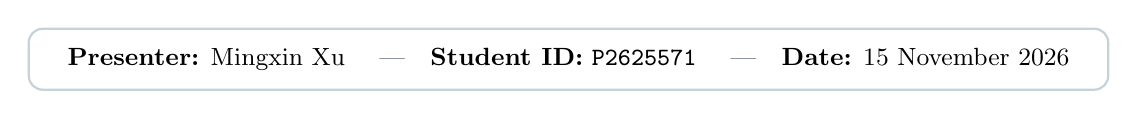
\begin{tikzpicture}
      \node[fill=white,draw=mpuBorder,rounded corners=5pt,line width=0.8pt,inner xsep=14pt,inner ysep=7pt] {
        \fontsize{9.5}{13}\selectfont
        \textbf{Presenter:} Mingxin Xu \quad\textcolor{mpuSlate}{|}\quad
        \textbf{Student ID:} \code{P2625571} \quad\textcolor{mpuSlate}{|}\quad
        \textbf{Date:} 15 November 2026
      };
    \end{tikzpicture}\\[0.28cm]

    {\fontsize{8.8}{11}\selectfont\color{mpuSlate}
      Repository (Code, Dataset, Artifact): \url{https://github.com/XuMingxin-web/Ferritin-AIDD8122}
    }
  \end{center}

  \vfill
  \begin{center}
  \setlength{\tabcolsep}{4pt}
  \begin{tabular}{@{}>{\centering\arraybackslash}p{0.22\textwidth}>{\centering\arraybackslash}p{0.22\textwidth}>{\centering\arraybackslash}p{0.22\textwidth}>{\centering\arraybackslash}p{0.26\textwidth}@{}}
    {\fontsize{8.2}{10}\selectfont\color{mpuNavy}\textbf{334} Curated Rows} &
    {\fontsize{8.2}{10}\selectfont\color{mpuTeal}\textbf{0.952} ROC-AUC} &
    {\fontsize{8.2}{10}\selectfont\color{mpuOrange}\textbf{100\%} Sign Acc.} &
    {\fontsize{8.2}{10}\selectfont\color{mpuNavy}\textbf{$p \in [0.0007, 0.033]$}} \\[-2pt]
    {\fontsize{7.4}{9}\selectfont\color{mpuSlate}(240 Unique Mutants)} &
    {\fontsize{7.4}{9}\selectfont\color{mpuSlate}(Unseen \code{S5} Cohort)} &
    {\fontsize{7.4}{9}\selectfont\color{mpuSlate}(12-mer Zero-Shot \code{S2})} &
    {\fontsize{7.4}{9}\selectfont\color{mpuSlate}(Wilcoxon Wins, $N=47$)}
  \end{tabular}
  \end{center}
  \vspace*{0.10cm}
\end{frame}

% =========================================================================
% SLIDE 2: PROBLEM STATEMENT & MOTIVATION
% =========================================================================
\begin{frame}{Motivation: Why Off-the-Shelf Stability Models Fail on Ferritins}
  \framesubtitle{Public database void, quaternary interface blindness, and evolutionary-stability inversion}

  \begin{columns}[T,totalwidth=\textwidth]
    \begin{column}{0.55\textwidth}
      \begin{block}{\footnotesize 1. Public Database Void (17 Audited Corpora)}
        \fontsize{7.8}{9.8}\selectfont
        \begin{itemize}
          \item Ferritins form \textbf{24-mer octahedral} ($\approx 12\text{ nm}$) \& \textbf{12-mer tetrahedral} Dps nanocages for drug delivery, biocatalysis, \& vaccines.
          \item Programmatic audit of FireProtDB (41.1M SQL lines), ThermoMutDB (13,337 rows), GeoStab (14,340), ProteinGym, Tsuboyama, \& MaveDB found \textbf{0 natural ferritin point-mutant $\DTm$ records}.
          \item ProThermDB held only 4 mislabeled EBNA1--HuHF fusions; NTU thesis tables invert sign ($\DTm^{\text{thesis}} = T_m^{\text{WT}} - T_m^{\text{mut}}$).
        \end{itemize}
      \end{block}

      \vspace*{-2pt}
      \begin{alertblock}{\footnotesize 2. Biophysical \& Evolutionary Inversion}
        \fontsize{7.8}{9.8}\selectfont
        \begin{itemize}
          \item \textbf{Monomer blindness:} Stability originates at $C_2/C_3/C_4$ interfaces (\code{MjFer D132R} $-18.0^\circ\text{C}$; \code{CgFer D120G} $+13.0^\circ\text{C}$).
          \item \textbf{Evolutionary conflict:} Pore/catalytic residues are conserved for iron flux---\code{ESM-2 LLR} inverts correlation ($r=-0.363$).
        \end{itemize}
      \end{alertblock}
    \end{column}

    \begin{column}{0.43\textwidth}
      \begin{exampleblock}{\footnotesize Baseline Failure on \texttt{S1\_PairedCore23} ($n=23$)}
        \centering
        \setlength{\tabcolsep}{4pt}
        \fontsize{7.5}{9.5}\selectfont
        \begin{tabular}{@{}lcc@{}}
          \toprule
          \textbf{Method} & \textbf{MAE ($^\circ$C)} & \textbf{Pearson $r$} \\
          \midrule
          Zero Baseline ($\DTm=0$) & 9.91 & --- \\
          ESM-2 WT-Marginal LLR & 12.22 & \textcolor{mpuRed}{$-0.363$} \\
          FoldX Monomer & 10.19 & \textcolor{mpuRed}{$-0.195$} \\
          Mono GeoDTm-3D ($k=32$) & 10.04 & $-0.068$ \\
          \midrule
          FoldX Cage Eff. (7-mer) & 9.39 & \textcolor{mpuTeal}{$+0.222$} \\
          FoldX $A{\leftrightarrow}C$ Binding & 9.44 & \textcolor{mpuTeal}{$+0.312$} \\
          \textbf{GeoHybrid (S1 LOPO)} & \textbf{8.58} & \textbf{\textcolor{mpuNavy}{$+0.375$}} \\
          \bottomrule
        \end{tabular}
      \end{exampleblock}

      \vspace*{2pt}
      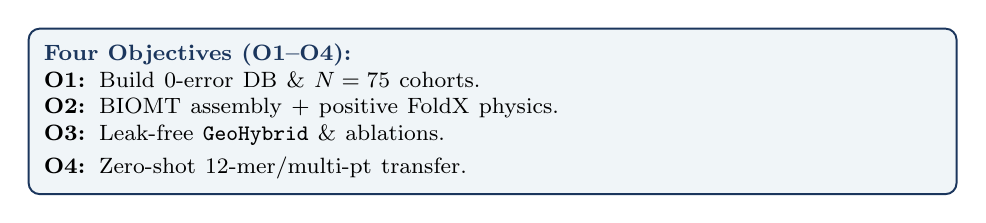
\begin{tikzpicture}
        \node[fill=mpuLight,draw=mpuNavy,rounded corners=4pt,line width=0.7pt,text width=0.94\linewidth,inner sep=5.5pt] {
          \fontsize{7.6}{9.6}\selectfont
          \textbf{\color{mpuNavy}Four Objectives (O1--O4):}\\
          \textbf{O1:} Build 0-error DB \& $N=75$ cohorts.\\
          \textbf{O2:} BIOMT assembly + positive FoldX physics.\\
          \textbf{O3:} Leak-free \code{GeoHybrid} \& ablations.\\
          \textbf{O4:} Zero-shot 12-mer/multi-pt transfer.
        };
      \end{tikzpicture}
    \end{column}
  \end{columns}
\end{frame}

% =========================================================================
% SLIDE 3: CURATED DATABASE & COHORTS
% =========================================================================
\begin{frame}{Objective 1: 17-Source Curation, Sign Standardization \& Cohorts}
  \framesubtitle{334 validated condition-rows / 240 unique mutants (0 validation errors) and 75 structural cases}

  \begin{columns}[c,totalwidth=\textwidth]
    \begin{column}{0.39\textwidth}
      \begin{block}{\footnotesize Database Hygiene \& Reconciliation}
        \fontsize{7.7}{9.7}\selectfont
        \begin{itemize}
          \item Triangulated 269 PMC full texts, 7,083 Europe PMC, 1,856 PubMed XML, \& DR-NTU 48015.
          \item Standardized $\DTm = T_m^{\text{mut}} - T_m^{\text{WT}}$; logged 165 paywalled items separately.
          \item Restored artifacts via FoldX (\code{HuHF 2FHA K86Q}, \code{MjFer 6A4U R177H}).
          \item \code{validate_deliverables.py}: \textbf{334 rows / 240 unique, 0 errors}.
        \end{itemize}
      \end{block}

      \vspace*{2pt}
      \centering
      \setlength{\tabcolsep}{3.5pt}
      \fontsize{7.3}{9.1}\selectfont
      \begin{tabular}{@{}llr@{}}
        \toprule
        \textbf{Cohort} & \textbf{Symmetry / Role} & \textbf{$N$} \\
        \midrule
        \code{S1_All30} & 24-mer Train/CV & 30 \\
        \code{S2_EcDps} & 12-mer Zero-Shot & 8 \\
        \code{S3_Multi} & Multi-pt (9 exact+7 abst) & 16 \\
        \code{S4_Second} & Bimodal DSC Peak1/2 & 8 \\
        \code{S5_Direct} & Unseen Dir. (7+/6-) & 13 \\
        \bottomrule
      \end{tabular}
    \end{column}

    \begin{column}{0.59\textwidth}
      \centering
      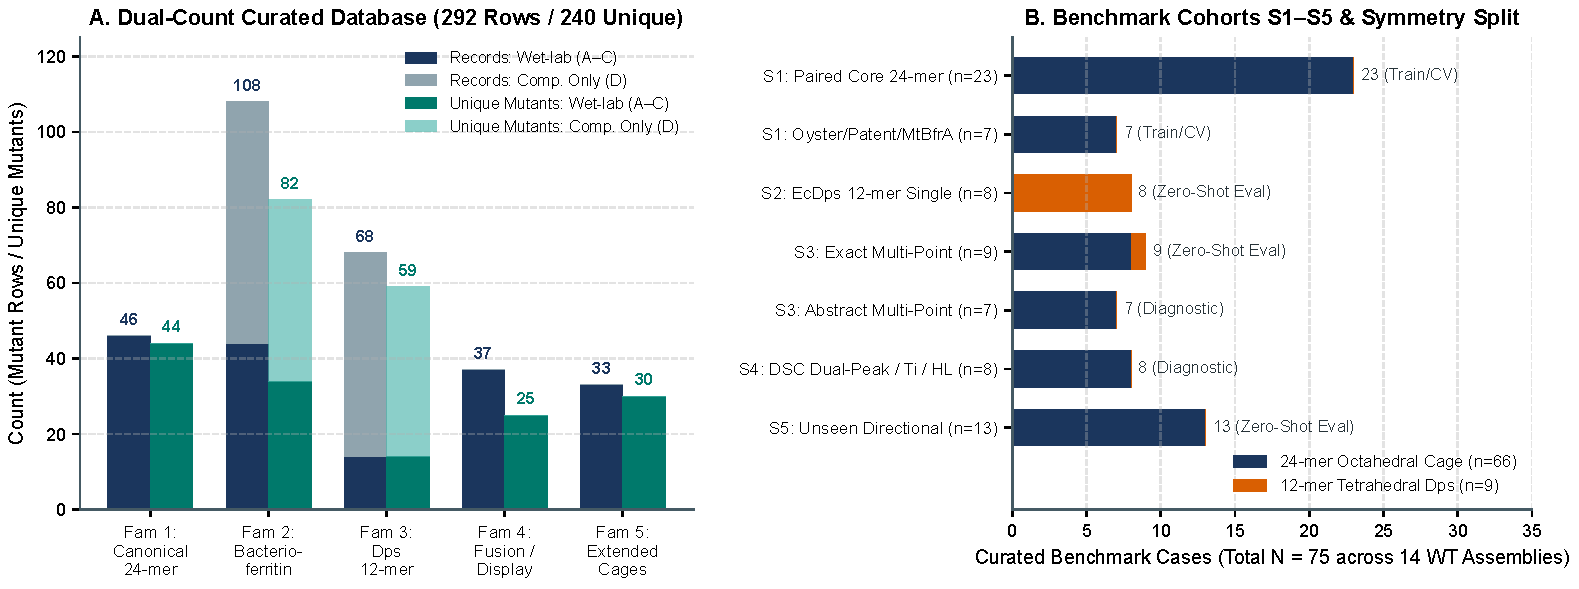
\includegraphics[width=\linewidth,height=5.6cm,keepaspectratio]{../figures/fig1_database_audit.pdf}
    \end{column}
  \end{columns}
\end{frame}

% =========================================================================
% SLIDE 4: BIOMT ASSEMBLY RECONSTRUCTION & VERIFICATION GATES
% =========================================================================
\begin{frame}{Objective 2: BIOMT 7-Chain Subcomplex \& Verification Gates}
  \framesubtitle{Symmetry-axis physics reconstruction and numerical parity checks prior to transfer}

  \centering
  \resizebox{0.99\textwidth}{!}{%
  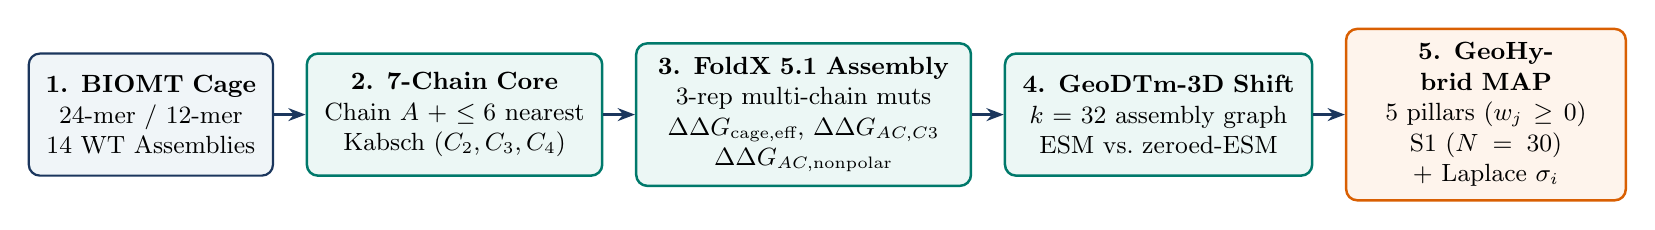
\begin{tikzpicture}[
    node distance=0.4cm,
    bnavy/.style={draw=mpuNavy,fill=mpuLight,rounded corners=4pt,line width=0.8pt,align=center,font=\small,inner sep=5pt,minimum height=1.55cm},
    bteal/.style={draw=mpuTeal,fill=mpuMint,rounded corners=4pt,line width=0.9pt,align=center,font=\small,inner sep=5pt,minimum height=1.55cm},
    borange/.style={draw=mpuOrange,fill=mpuPeach,rounded corners=4pt,line width=0.9pt,align=center,font=\small,inner sep=5pt,minimum height=1.55cm},
    arr/.style={-{Stealth[length=2.2mm]},thick,color=mpuNavy}
  ]
    \node[bnavy,text width=2.75cm] (a1) {\textbf{1. BIOMT Cage}\\24-mer / 12-mer\\14 WT Assemblies};
    \node[bteal,right=of a1,text width=3.4cm] (a2) {\textbf{2. 7-Chain Core}\\Chain $A$ + $\le 6$ nearest\\Kabsch ($C_2, C_3, C_4$)};
    \node[bteal,right=of a2,text width=3.9cm] (a3) {\textbf{3. FoldX 5.1 Assembly}\\3-rep multi-chain muts\\$\DDG_{\text{cage,eff}},\,\DDG_{AC,C3}$\\$\DDG_{AC,\text{nonpolar}}$};
    \node[bteal,right=of a3,text width=3.55cm] (a4) {\textbf{4. GeoDTm-3D Shift}\\$k=32$ assembly graph\\ESM vs.\ zeroed-ESM};
    \node[borange,right=of a4,text width=3.2cm] (a5) {\textbf{5. GeoHybrid MAP}\\5 pillars ($w_j \ge 0$)\\S1 ($N=30$) + Laplace $\sigma_i$};
    \draw[arr] (a1) -- (a2);
    \draw[arr] (a2) -- (a3);
    \draw[arr] (a3) -- (a4);
    \draw[arr] (a4) -- (a5);
  \end{tikzpicture}%
  }

  \vspace{0.25cm}
  \begin{columns}[T,totalwidth=\textwidth]
    \begin{column}{0.32\textwidth}
      \begin{block}{\footnotesize GeoDTm-3D Parity Gate}
        \fontsize{7.8}{10}\selectfont
        \begin{itemize}
          \item Official \code{S571} test ($n=571$): $r=0.4673$, $\rho=0.5096$, $\text{MAE}=5.308^\circ\text{C}$ (vs.\ $6.280^\circ\text{C}$ zero).
          \item \code{1CTS_H274R}: exact $0.0^\circ\text{C}$ diff.
          \item \code{EcBfr_R30A} script parity: $1.73\times 10^{-6\,^\circ}\text{C}$.
        \end{itemize}
      \end{block}
    \end{column}
    \begin{column}{0.32\textwidth}
      \begin{exampleblock}{\footnotesize FoldX 5.1 Numerical Gate}
        \fontsize{7.8}{10}\selectfont
        \begin{itemize}
          \item Stratified 36-case \code{S571} author comparison: \textbf{$r=0.99958$}.
          \item Median diff: $2.64\times 10^{-5}\text{ kcal/mol}$.
          \item 100\% directional sign agreement.
        \end{itemize}
      \end{exampleblock}
    \end{column}
    \begin{column}{0.32\textwidth}
      \begin{alertblock}{\footnotesize Symmetry Axis Gate}
        \fontsize{7.8}{10}\selectfont
        \begin{itemize}
          \item Rigid-body Kabsch resolves $C_2$ ($180^\circ$), $C_3$ ($120^\circ$), $C_4$ ($90^\circ$).
          \item 12-mer \code{EcDps} (\code{1F33}) passes 0 $C_4$ partners check.
          \item Unifies 24-mer \& 12-mer inputs.
        \end{itemize}
      \end{alertblock}
    \end{column}
  \end{columns}
\end{frame}

% =========================================================================
% SLIDE 5: FERRITIN-GEOHYBRID ARCHITECTURE & CV DESIGN
% =========================================================================
\begin{frame}{Methodology: Decoupling ESM Bias via Prior-Anchored Huber MAP}
  \framesubtitle{Constrained 5-pillar estimator preventing sign-flip collapse under small sample size ($N=30$)}

  \begin{columns}[T,totalwidth=\textwidth]
    \begin{column}{0.48\textwidth}
      \begin{block}{\footnotesize Five Standardized Physical Pillars ($\tilde{\mathbf{x}}_i \in \mathbb{R}^5$)}
        \fontsize{7.9}{10.2}\selectfont
        \begin{enumerate}
          \item \code{geo_asm_k32}: 7-chain assembly \code{GeoDTm-3D}.
          \item \code{neg_fx_cage_ddg_eff}:\\ $0.5\,\DDG_{\text{sub/chain}} + 0.5\,(\frac{1}{2}\DDG_{AC,\text{bind}})$.
          \item \code{neg_fx_ac_ddg_bind_c3}: $C_3$ channel binding.
          \item \code{neg_fx_ac_ddg_bind_nonpolar}: vdW + solv\_hyd.
          \item \code{neg_geo_asm_enc_shift_k32}:\\ $-\bigl[\text{GeoDTm}^{\text{asm}}(\text{ESM}) - \text{GeoDTm}^{\text{asm}}(\text{zero})\bigr]$\\
          {\color{mpuSlate}(removes evolutionary penalty on functional pores)}.
        \end{enumerate}
      \end{block}
    \end{column}

    \begin{column}{0.49\textwidth}
      \begin{exampleblock}{\footnotesize \texttt{NonNegHuberMAPRegressor} Objective}
        \fontsize{7.9}{10.1}\selectfont
        \vspace*{-0.15cm}
        \[
          \min_{b_0 \in \mathbb{R},\;\mathbf{w} \ge \mathbf{0}}\;\sum_{i=1}^{N}\ell_{\delta}\!\left(y_i - b_0 - \mathbf{w}^\top\tilde{\mathbf{x}}_i\right) + \frac{\alpha}{2}\sum_{j=1}^{5}\left(w_j - w_{\text{prior}}\right)^2
        \]
        \vspace*{-0.22cm}
        \begin{itemize}
          \item \textbf{Huber $\delta = 8.0^\circ\text{C}$:} resists $+26.3^\circ\text{C}$ extreme outliers.
          \item \textbf{Prior ($w_j \ge 0$, $w_{\text{prior}}=1.0$, $\alpha=80.0$):} selected via nested \code{GroupKFold}; blocks sign flipping.
          \item \textbf{IRLS Laplace $\sigma_i$:} predictive uncertainty.
        \end{itemize}
      \end{exampleblock}

      \vspace*{2pt}
      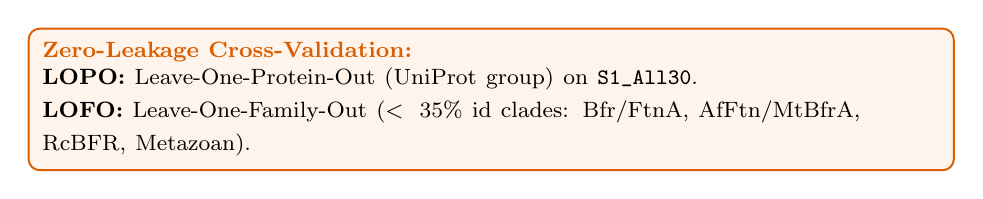
\begin{tikzpicture}
        \node[fill=mpuPeach,draw=mpuOrange,rounded corners=4pt,line width=0.7pt,text width=0.94\linewidth,inner sep=5pt] {
          \fontsize{7.6}{9.6}\selectfont
          \textbf{\color{mpuOrange}Zero-Leakage Cross-Validation:}\\
          \textbf{LOPO:} Leave-One-Protein-Out (UniProt group) on \code{S1_All30}.\\
          \textbf{LOFO:} Leave-One-Family-Out ($<35\%$ id clades: Bfr/FtnA, AfFtn/MtBfrA, RcBFR, Metazoan).
        };
      \end{tikzpicture}
    \end{column}
  \end{columns}
\end{frame}

% =========================================================================
% SLIDE 6: S1 BASELINES, CV & WEIGHT STABILITY
% =========================================================================
\begin{frame}{Results (RQ2--RQ3): Out-of-Fold Generalization on \texttt{S1\_All30}}
  \framesubtitle{Significant LOPO ($r=+0.375$) and $<35\%$ identity LOFO ($r=+0.394$) with 100\% positive weights}

  \centering
  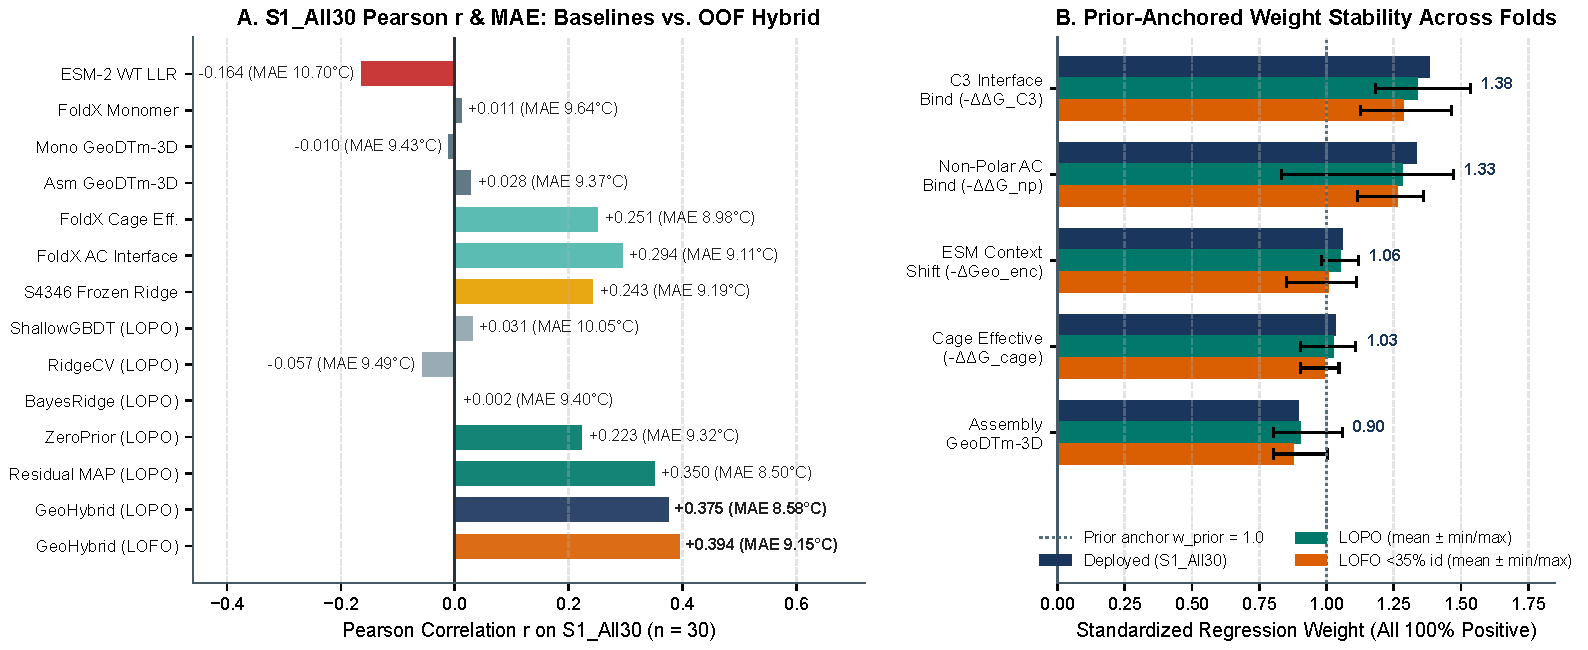
\includegraphics[width=0.96\textwidth,height=4.45cm,keepaspectratio]{../figures/fig2_s1_baselines_and_cv.pdf}

  \vspace{0.12cm}
  \begin{columns}[T,totalwidth=\textwidth]
    \begin{column}{0.32\textwidth}
      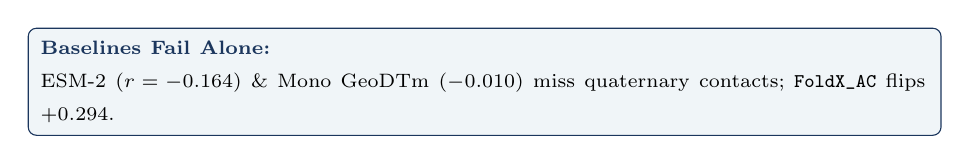
\begin{tikzpicture}
        \node[fill=mpuLight,draw=mpuNavy,rounded corners=3pt,text width=0.93\linewidth,inner sep=4.5pt] {
          \fontsize{7.4}{9.3}\selectfont
          \textbf{\color{mpuNavy}Baselines Fail Alone:}\\
          ESM-2 ($r=-0.164$) \& Mono GeoDTm ($-0.010$) miss quaternary contacts; \code{FoldX_AC} flips $+0.294$.
        };
      \end{tikzpicture}
    \end{column}
    \begin{column}{0.32\textwidth}
      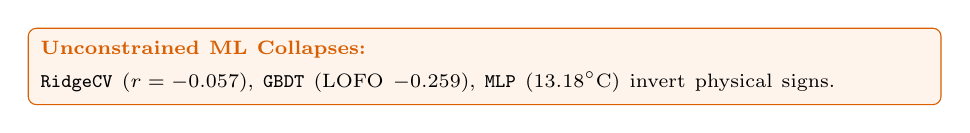
\begin{tikzpicture}
        \node[fill=mpuPeach,draw=mpuOrange,rounded corners=3pt,text width=0.93\linewidth,inner sep=4.5pt] {
          \fontsize{7.4}{9.3}\selectfont
          \textbf{\color{mpuOrange}Unconstrained ML Collapses:}\\
          \code{RidgeCV} ($r=-0.057$), \code{GBDT} (LOFO $-0.259$), \code{MLP} ($13.18^\circ\text{C}$) invert physical signs.
        };
      \end{tikzpicture}
    \end{column}
    \begin{column}{0.33\textwidth}
      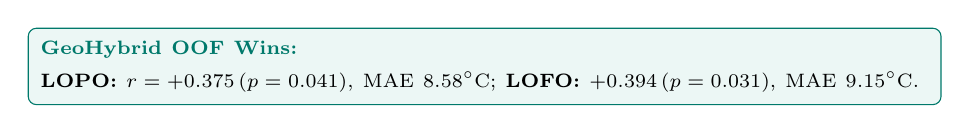
\begin{tikzpicture}
        \node[fill=mpuMint,draw=mpuTeal,rounded corners=3pt,text width=0.93\linewidth,inner sep=4.5pt] {
          \fontsize{7.4}{9.3}\selectfont
          \textbf{\color{mpuTeal}GeoHybrid OOF Wins:}\\
          \textbf{LOPO:} $r=+0.375\,(p=0.041)$, MAE $8.58^\circ\text{C}$; \textbf{LOFO:} $+0.394\,(p=0.031)$, MAE $9.15^\circ\text{C}$.
        };
      \end{tikzpicture}
    \end{column}
  \end{columns}
\end{frame}

% =========================================================================
% SLIDE 7: MECHANISTIC ABLATIONS & S5 ROC
% =========================================================================
\begin{frame}{Results (RQ3): Stepwise Ablations (\texttt{Ab1}--\texttt{Ab6}) \& Unseen \texttt{S5} ROC}
  \framesubtitle{Monotonic LOFO gain from monomer to 5-pillar GeoHybrid; excluding raw ESM-2 LLR prevents degradation}

  \centering
  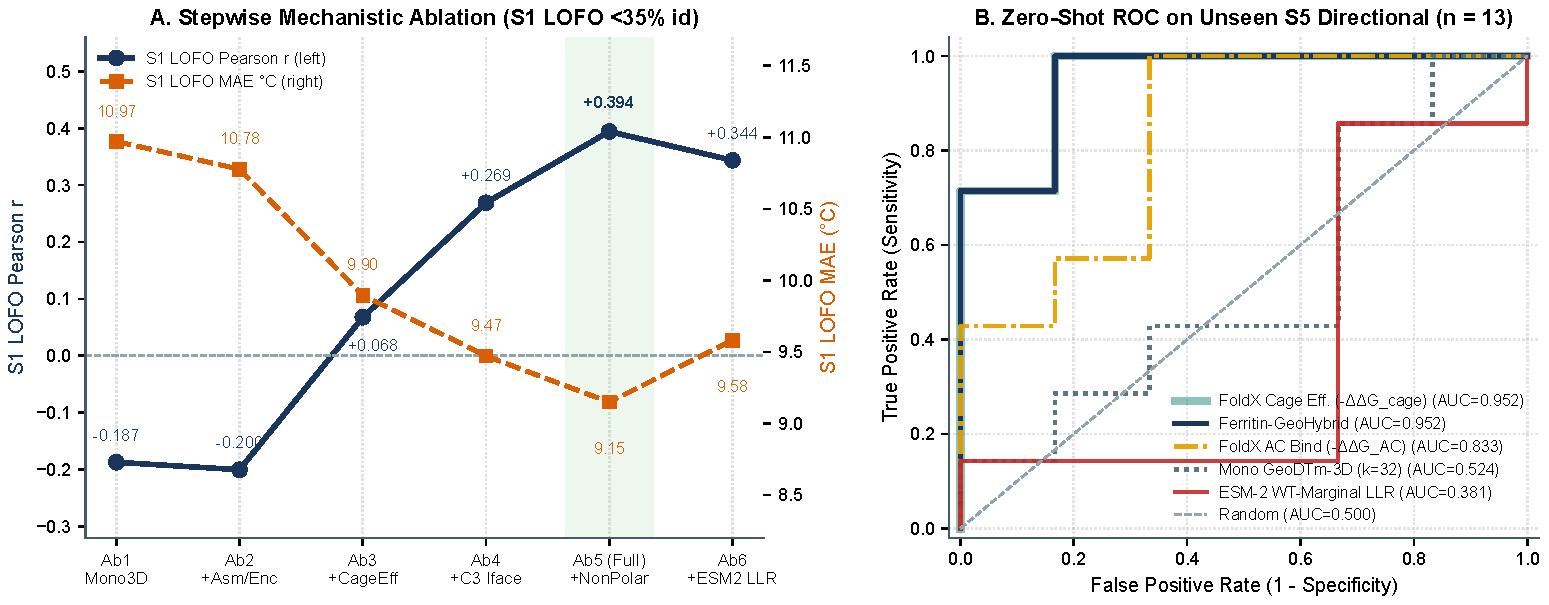
\includegraphics[width=0.96\textwidth,height=4.4cm,keepaspectratio]{../figures/fig3_ablation_and_roc.pdf}

  \vspace{0.10cm}
  \begin{columns}[T,totalwidth=\textwidth]
    \begin{column}{0.49\textwidth}
      \begin{block}{\footnotesize Monotonic Causality Across Ablations (\texttt{Ab1}--\texttt{Ab6})}
        \fontsize{7.6}{9.6}\selectfont
        \begin{itemize}
          \item \textbf{LOFO $r$:} $-0.187$ (\code{Ab1}) $\to +0.068$ (\code{Ab3}) $\to +0.269$ (\code{Ab4}) $\to \mathbf{+0.394}$ (\code{Ab5}); MAE $10.97 \to \mathbf{9.15^\circ\text{C}}$.
          \item Re-adding raw \code{ESM-2 LLR} (\code{Ab6}) hurts LOFO ($+0.344$, MAE $9.58^\circ\text{C}$) \& drops \code{S5} AUC ($0.952 \to 0.833$).
        \end{itemize}
      \end{block}
    \end{column}
    \begin{column}{0.49\textwidth}
      \begin{exampleblock}{\footnotesize Unseen Directional Cohort \texttt{S5} ($N=13$: 7 Pos / 6 Neg)}
        \fontsize{7.6}{9.6}\selectfont
        \begin{itemize}
          \item \textbf{Ferritin-GeoHybrid:} $\mathbf{\text{ROC-AUC} = 0.952}$ (Mann--Whitney $U=40.0$, $p=0.0023$).
          \item Beats Mono/Asm \code{GeoDTm-3D} ($0.524$), \code{ESM-2 LLR} ($0.381$), \& \code{BayesianRidge_FreeSign7} ($0.643$).
        \end{itemize}
      \end{exampleblock}
    \end{column}
  \end{columns}
\end{frame}

% =========================================================================
% SLIDE 8: ZERO-SHOT CROSS-SYMMETRY & MULTI-POINT TRANSFER
% =========================================================================
\begin{frame}{Results (RQ4): Zero-Shot Transfer (\texttt{S2}, \texttt{S3}, Pooled \texttt{N=47})}
  \framesubtitle{Frozen 24-mer single-mutant model transfers to 12-mer EcDps and multi-point assemblies}

  \begin{columns}[c,totalwidth=\textwidth]
    \begin{column}{0.66\textwidth}
      \centering
      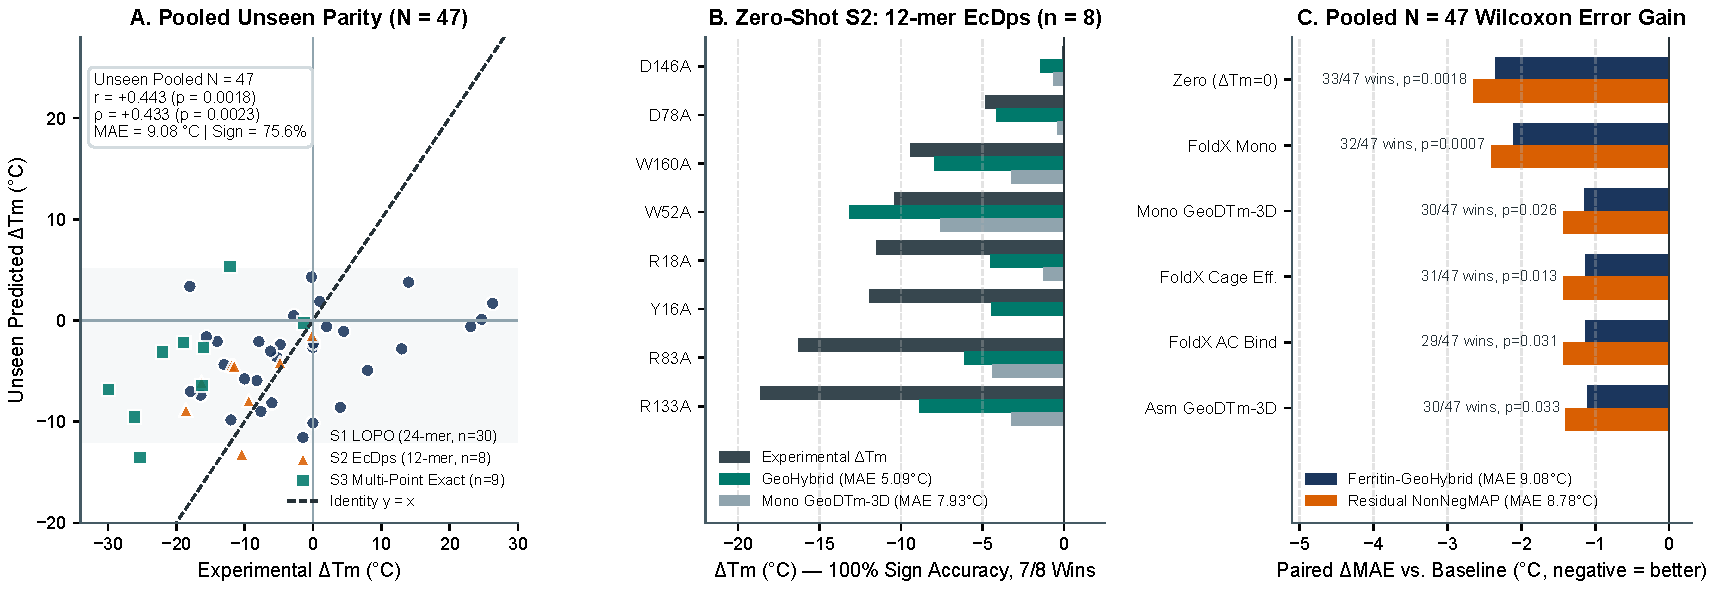
\includegraphics[width=\linewidth,height=5.55cm,keepaspectratio]{../figures/fig4_zeroshot_transfer.pdf}
    \end{column}

    \begin{column}{0.32\textwidth}
      \begin{exampleblock}{\footnotesize \texttt{S2} 12-mer \textit{EcDps} ($n=8$)}
        \fontsize{7.5}{9.4}\selectfont
        \textbf{MAE:} $5.09^\circ\text{C}$ (vs.\ $10.38^\circ\text{C}$ Zero)\\
        \textbf{Sign Acc:} \textbf{100\%} (8/8); $r=+0.505$\\
        Beats Mono ($p=0.0234$) \& FoldX\_mono ($p=0.0156$); 75\% $1\sigma$ / 100\% $2\sigma$.
      \end{exampleblock}

      \vspace*{-3pt}
      \begin{block}{\footnotesize \texttt{S3\_Exact9} Multi-Pt ($n=9$)}
        \fontsize{7.5}{9.4}\selectfont
        \textbf{Spearman $\rho$:} \textbf{$+0.833$ ($p=0.0053$)}\\
        \textbf{Pearson $r$:} $+0.678$ ($p=0.0447$)\\
        88.9\% sign; MAE $14.29^\circ\text{C}$ ($p=0.0391$); Residual $12.91^\circ\text{C}$.
      \end{block}

      \vspace*{-3pt}
      \begin{alertblock}{\footnotesize Pooled Unseen ($N=47$)}
        \fontsize{7.5}{9.4}\selectfont
        \textbf{$r=+0.443$ ($p=0.0018$)}, $\rho=+0.433$\\
        \textbf{MAE:} $9.08^\circ\text{C}$ (Residual $8.78^\circ\text{C}$)\\
        Beats \textbf{all 6 baselines} via Wilcoxon ($p=0.0007\text{--}0.0330$).
      \end{alertblock}
    \end{column}
  \end{columns}
\end{frame}

% =========================================================================
% SLIDE 9: BIOPHYSICAL ERROR AUDIT & S4 DIAGNOSTICS
% =========================================================================
\begin{frame}{Error Audit \& Multi-State Boundaries (\texttt{S1 LOPO} \& \texttt{S4})}
  \framesubtitle{Understanding rigid-backbone sterics, cofactors, and bimodal DSC cage dissociation}

  \centering
  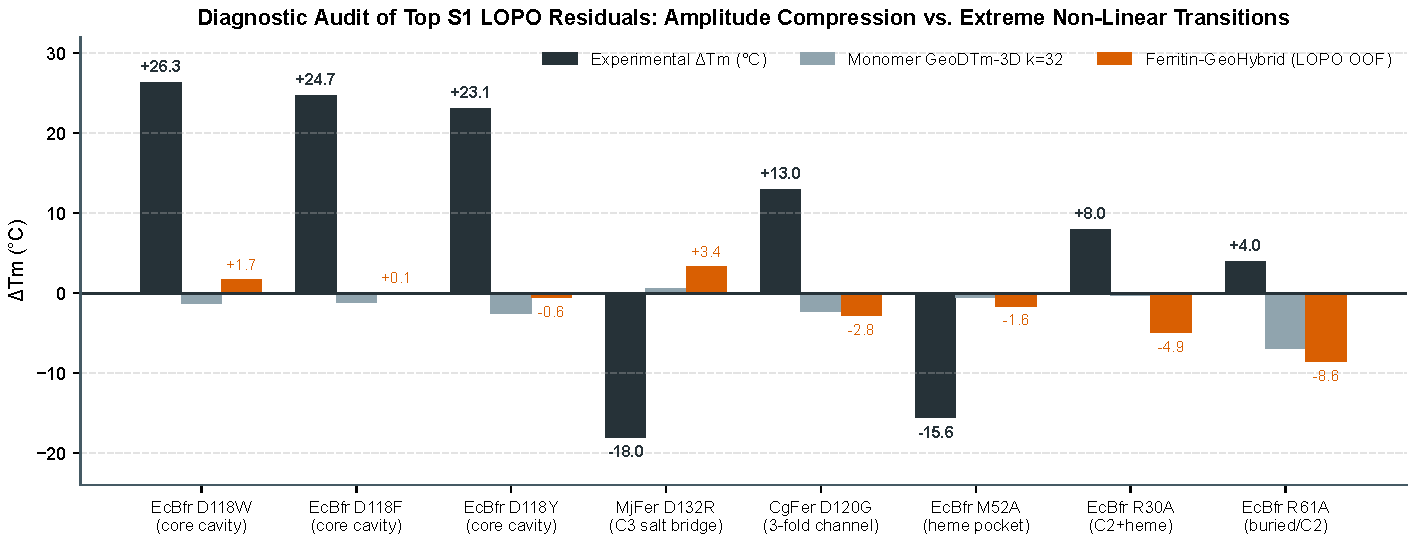
\includegraphics[width=0.92\textwidth,height=4.05cm,keepaspectratio]{../figures/fig5_error_audit.pdf}

  \vspace{0.10cm}
  \begin{columns}[T,totalwidth=\textwidth]
    \begin{column}{0.32\textwidth}
      \begin{alertblock}{\footnotesize 1. Cavity Plugging (\texttt{D118W/F/Y})}
        \fontsize{7.5}{9.4}\selectfont
        $+23.1$ to $+26.3^\circ\text{C}$ observed vs.\ compressed OOF predictions ($+1.7$ to $-0.6^\circ\text{C}$). Rigid \code{FoldX} over-penalizes bulky aromatics in buried pockets.
      \end{alertblock}
    \end{column}
    \begin{column}{0.33\textwidth}
      \begin{block}{\footnotesize 2. Channels \& Cofactors}
        \fontsize{7.5}{9.4}\selectfont
        \code{MjFer D132R} ($-18.0^\circ\text{C}$), \code{CgFer D120G} ($+13.0^\circ\text{C}$), and heme-proximal \code{EcBfr M52A}/\code{R30A} involve backbone/cofactor cooperativity.
      \end{block}
    \end{column}
    \begin{column}{0.32\textwidth}
      \begin{exampleblock}{\footnotesize 3. Bimodal DSC (\texttt{S4}, $n=8$)}
        \fontsize{7.5}{9.4}\selectfont
        \code{EcBfr} splits into cage dissociation (\code{Peak1}) \& subunit unfolding (\code{Peak2}), causing inversion ($r=-0.193$) under single-scalar $\DTm$.
      \end{exampleblock}
    \end{column}
  \end{columns}
\end{frame}

% =========================================================================
% SLIDE 10: STRENGTHS, LIMITATIONS & FUTURE ROADMAP
% =========================================================================
\begin{frame}{Critical Evaluation: Strengths, Limitations \& Roadmap}
  \framesubtitle{Balancing interpretability and small-sample guarantees against next-generation horizons}

  \begin{columns}[T,totalwidth=\textwidth]
    \begin{column}{0.48\textwidth}
      \begin{exampleblock}{\footnotesize Key Strengths \& Contributions}
        \fontsize{8.1}{10.5}\selectfont
        \begin{itemize}
          \item \textbf{Zero-error benchmark curation:} 334 rows / 240 unique mutants fixing sign inversions \& artifacts across 17 corpora.
          \item \textbf{Full interpretability:} 5 grounded pillars with 100\% positive weights invariant across every LOPO/LOFO fold.
          \item \textbf{Verified symmetry transfer:} 24-mer training transfers zero-shot to 12-mer \textit{EcDps} (100\% sign acc.) \& multi-point cages ($\rho=0.833$).
          \item \textbf{Deterministic reproducibility:} Unit tests, parity gates ($r=0.99958$), \& artifact (\code{169b357c...}).
        \end{itemize}
      \end{exampleblock}
    \end{column}

    \begin{column}{0.49\textwidth}
      \begin{alertblock}{\footnotesize Current Limitations \& Future Roadmap}
        \fontsize{8.1}{10.5}\selectfont
        \begin{itemize}
          \item \textbf{Amplitude compression bias:} Shrinkage ($\alpha=80.0$) compresses extreme shifts ($+2.47^\circ\text{C}$ bias on Pooled $N=47$).\\
          {\color{mpuSlate}\textit{$\rightarrow$ Roadmap: Non-linear / quantile residual heads.}}
          \item \textbf{Rigid backbone \& missing cofactors:} \code{FoldX} omits heme-$b$/di-iron metals \& $C_3$ loop plasticity.\\
          {\color{mpuSlate}\textit{$\rightarrow$ Roadmap: Cofactor-retaining MD / Flex ddG.}}
          \item \textbf{Small supervised training size ($N=30$):}\\
          {\color{mpuSlate}\textit{$\rightarrow$ Roadmap: Recover 29 prioritized ESI/paywalled sources to reach $N \ge 80$.}}
        \end{itemize}
      \end{alertblock}
    \end{column}
  \end{columns}
\end{frame}

% =========================================================================
% SLIDE 11: CONCLUSIONS & REPRODUCIBILITY CHECKLIST
% =========================================================================
\begin{frame}{Conclusions \& Public GitHub Reproducibility}
  \framesubtitle{All four research objectives achieved with open data, verified code, and frozen artifact}

  \begin{columns}[T,totalwidth=\textwidth]
    \begin{column}{0.55\textwidth}
      \begin{block}{\footnotesize Summary of Achievements (O1--O4)}
        \fontsize{8.0}{10.3}\selectfont
        \begin{enumerate}
          \item \textbf{Database Infrastructure (O1):} Exposed total omission across 17 stability DBs; built 334-row / 240-unique benchmark (0 errors).
          \item \textbf{Assembly Physics (O2):} BIOMT 7-chain subcomplexes + Kabsch $C_2/C_3/C_4$ decomposition flip correlations positive.
          \item \textbf{Hybrid Modeling (O3):} \code{Ferritin-GeoHybrid} beats baselines \& unconstrained ML on LOPO ($r=+0.375$) \& LOFO ($r=+0.394$), proven by \code{Ab1}--\code{Ab5}.
          \item \textbf{Zero-Shot Transfer (O4):} Generalizes to 12-mer \textit{EcDps} ($5.09^\circ\text{C}$), multi-point \code{S3} ($\rho=0.833$), \code{S5} ($\text{AUC}=0.952$), \& Pooled $N=47$ ($p=0.0018$).
        \end{enumerate}
      \end{block}
    \end{column}

    \begin{column}{0.42\textwidth}
      \begin{exampleblock}{\footnotesize GitHub Repository Organization}
        \fontsize{7.5}{9.6}\selectfont
        \begin{itemize}
          \item \textbf{Repo:} \href{https://github.com/XuMingxin-web/Ferritin-AIDD8122}{\texttt{XuMingxin-web/Ferritin-AIDD8122}}
          \item \code{scripts/build_ferritin_mt_db.py} \& \code{validate_deliverables.py}
          \item \code{research/src/assembly_builder.py}, \code{foldx_assembly.py}, \code{geodtm_assembly_adapter.py}, \code{hybrid_model.py}
          \item \code{research/models/ferritin_geohybrid.joblib}
          \item \code{research/tests/test_hybrid_model.py} \& \code{test_ferritin_pipeline.py}
          \item \code{docs/report/}, \code{docs/slides/}, \code{docs/figures/}
        \end{itemize}
      \end{exampleblock}
    \end{column}
  \end{columns}
\end{frame}

% =========================================================================
% SLIDE 12: THANK YOU & Q&A
% =========================================================================
\begin{frame}[plain]
  \begin{tikzpicture}[remember picture,overlay]
    \fill[mpuNavy] (current page.north west) rectangle ([yshift=-0.22cm]current page.north east);
    \fill[mpuGreen] ([yshift=-0.22cm]current page.north west) rectangle ([yshift=-0.34cm]current page.north east);
    \fill[mpuLight] (current page.south west) rectangle ([yshift=1.0cm]current page.south east);
    \draw[mpuBorder,line width=0.6pt] ([yshift=1.0cm]current page.south west) -- ([yshift=1.0cm]current page.south east);
  \end{tikzpicture}

  \vspace*{0.85cm}
  \begin{center}
    
\includegraphics[height=1.65cm]{../assets/mpu_logo.png}\\[0.4cm]
    {\fontsize{23}{27}\selectfont\bfseries\color{mpuNavy} Thank You for Your Attention!}\\[0.22cm]
    {\fontsize{12.5}{15}\selectfont\color{mpuTeal}\bfseries Questions \& Discussion (5-Minute Q\&A)}\\[0.48cm]

    
\begin{tikzpicture}
      \node[fill=mpuLight,draw=mpuBorder,rounded corners=5pt,inner xsep=18pt,inner ysep=9pt,align=center] {
        \fontsize{9.2}{13}\selectfont
        \textbf{Mingxin Xu} (Student ID: \code{P2625571})\\
        Faculty of Applied Sciences --- Macao Polytechnic University\\
        \textbf{Repository:} \url{https://github.com/XuMingxin-web/Ferritin-AIDD8122}
      };
    \end{tikzpicture}
  \end{center}
\end{frame}

% =========================================================================
% Q&A BACKUP SLIDES
% =========================================================================
\backupbegin

% BACKUP A: QUANTITATIVE BENCHMARK TABLES
\begin{frame}{Backup A: Complete Ablation (\texttt{Ab1}--\texttt{Ab6}) \& Pooled \texttt{N=47} Statistics}
  \framesubtitle{Quantitative metrics across feature ablations and paired Wilcoxon signed-rank comparisons}

  \begin{columns}[T,totalwidth=\textwidth]
    \begin{column}{0.49\textwidth}
      \textbf{\footnotesize Table A1: Stepwise Ablation (\texttt{Ab1}--\texttt{Ab6})}\\[3pt]
      \setlength{\tabcolsep}{3pt}
      \fontsize{7.1}{9.1}\selectfont
      \begin{tabular}{@{}lcccc@{}}
        \toprule
        \textbf{Variant} & \textbf{LOPO $r$} & \textbf{LOFO MAE} & \textbf{LOFO $r$} & \textbf{S5 AUC} \\
        \midrule
        \code{Ab1}: Mono32 & $-0.331$ & 10.97 & $-0.187$ & 0.524 \\
        \code{Ab2}: +Asm+Shift & $+0.099$ & 10.78 & $-0.200$ & 0.667 \\
        \code{Ab3}: +CageEff & $+0.183$ & 9.90 & $+0.068$ & \textbf{0.976} \\
        \code{Ab4}: +$C_3$ Bind & $+0.278$ & 9.47 & $+0.269$ & 0.929 \\
        \textbf{\code{Ab5}: Full Hybrid} & \textbf{$+0.375$} & \textbf{9.15} & \textbf{$+0.394$} & \textbf{0.952} \\
        \code{Ab6}: +ESM2 LLR & $+0.331$ & 9.58 & $+0.344$ & 0.833 \\
        \bottomrule
      \end{tabular}
    \end{column}

    \begin{column}{0.49\textwidth}
      \textbf{\footnotesize Table A2: Pooled Unseen ($N=47$) Wilcoxon Tests}\\[3pt]
      \setlength{\tabcolsep}{3pt}
      \fontsize{7.1}{9.1}\selectfont
      \begin{tabular}{@{}lccc@{}}
        \toprule
        \textbf{Baseline ($N=47$)} & \textbf{Ref MAE} & \textbf{$\Delta$MAE (Wins)} & \textbf{Wilcoxon $p$} \\
        \midrule
        Zero ($\DTm=0$) & 11.43 & $-2.35$ (33/47) & 0.0018 \\
        FoldX Monomer & 11.19 & $-2.11$ (32/47) & 0.0007 \\
        Mono GeoDTm ($k=32$) & 10.22 & $-1.14$ (30/47) & 0.0257 \\
        Asm GeoDTm ($k=32$) & 10.18 & $-1.10$ (30/47) & 0.0330 \\
        FoldX $A{\leftrightarrow}C$ Bind & 10.21 & $-1.13$ (29/47) & 0.0312 \\
        FoldX Cage Eff. & 10.21 & $-1.13$ (31/47) & 0.0125 \\
        \bottomrule
      \end{tabular}
    \end{column}
  \end{columns}

  \vspace{0.22cm}
  \begin{block}{\footnotesize Residual NonNegMAP Companion Performance}
    \fontsize{7.7}{9.8}\selectfont
    Fixing \code{geo_asm_k32} coefficient at 1.0 and fitting the remaining 4 pillars to $(y_i - \text{geo\_asm\_k32})$ achieves \code{S1 LOPO MAE} $=8.50^\circ\text{C}$ ($r=+0.350$), \code{LOFO MAE} $=8.97^\circ\text{C}$ ($r=+0.391$), \code{S3 Exact9 MAE} $=12.91^\circ\text{C}$ ($r=+0.692$), and Pooled $N=47$ \code{MAE} $=8.78^\circ\text{C}$ ($r=+0.459, p=0.0012$, $\rho=+0.474$).
  \end{block}
\end{frame}

% BACKUP B: S4, S3 ABSTRACT SPLIT & REPRODUCIBILITY DETAILS
\begin{frame}{Backup B: Data Hygiene Edge Cases \& Validation Scope}
  \framesubtitle{Detailed accounting of sign standardization, excluded assays, and local verification environment}

  \begin{columns}[T,totalwidth=\textwidth]
    \begin{column}{0.48\textwidth}
      \begin{block}{\footnotesize Source Sign Conventions \& Exclusions}
        \fontsize{7.7}{9.8}\selectfont
        \begin{itemize}
          \item \textbf{Thesis sign flip:} Yang Zhang NTU thesis (DR-NTU 48015) defines $\DTm^{\text{thesis}} = T_m^{\text{WT}} - T_m^{\text{mut}}$; cross-checked against PMC 2010/2011 articles and unified to $\DTm = T_m^{\text{mut}} - T_m^{\text{WT}}$.
          \item \textbf{SKEMPI 2.0 exclusion:} 7 ferritin antibody-binding rows are SPR affinity ($K_d$ at $295\text{ K}$), not thermal $\DTm$, and are excluded cleanly.
          \item \textbf{Multi-point \texttt{S3\_All16}:} Full 16-case multi-point set keeps 93.8\% sign acc.\ (15/16), while exact-baseline \code{S3_Exact9} achieves $\rho=+0.833$.
        \end{itemize}
      \end{block}
    \end{column}

    \begin{column}{0.49\textwidth}
      \begin{exampleblock}{\footnotesize Local Verification \& Dependency Scope}
        \fontsize{7.7}{9.8}\selectfont
        \begin{itemize}
          \item \code{scripts/validate_deliverables.py}: passes across all 334 rows / 240 unique mutants (\textbf{0 errors}).
          \item \textbf{Precomputed artifacts preserved:} CSV/JSON predictions, CV splits, ablations, \& \code{ferritin_geohybrid.joblib} (SHA-256 \code{169b357c...}).
          \item \textbf{Full test execution:} \code{test_hybrid_model.py} requires \code{scikit-learn} \& \code{joblib} (\code{requirements.txt}); core DB/BIOMT/metric modules run on base NumPy/Pandas/SciPy.
          \item \textbf{Excluded caches (.gitignore):} 312 MB raw intermediates excluded for a clean, lightweight GitHub push.
        \end{itemize}
      \end{exampleblock}
    \end{column}
  \end{columns}
\end{frame}

\end{document}
